% \documentclass[tikz,convert={outfile=\jobname.svg}]{standalone}
\documentclass[tikz]{standalone}
\usetikzlibrary{shapes.geometric, arrows}
\begin{document}
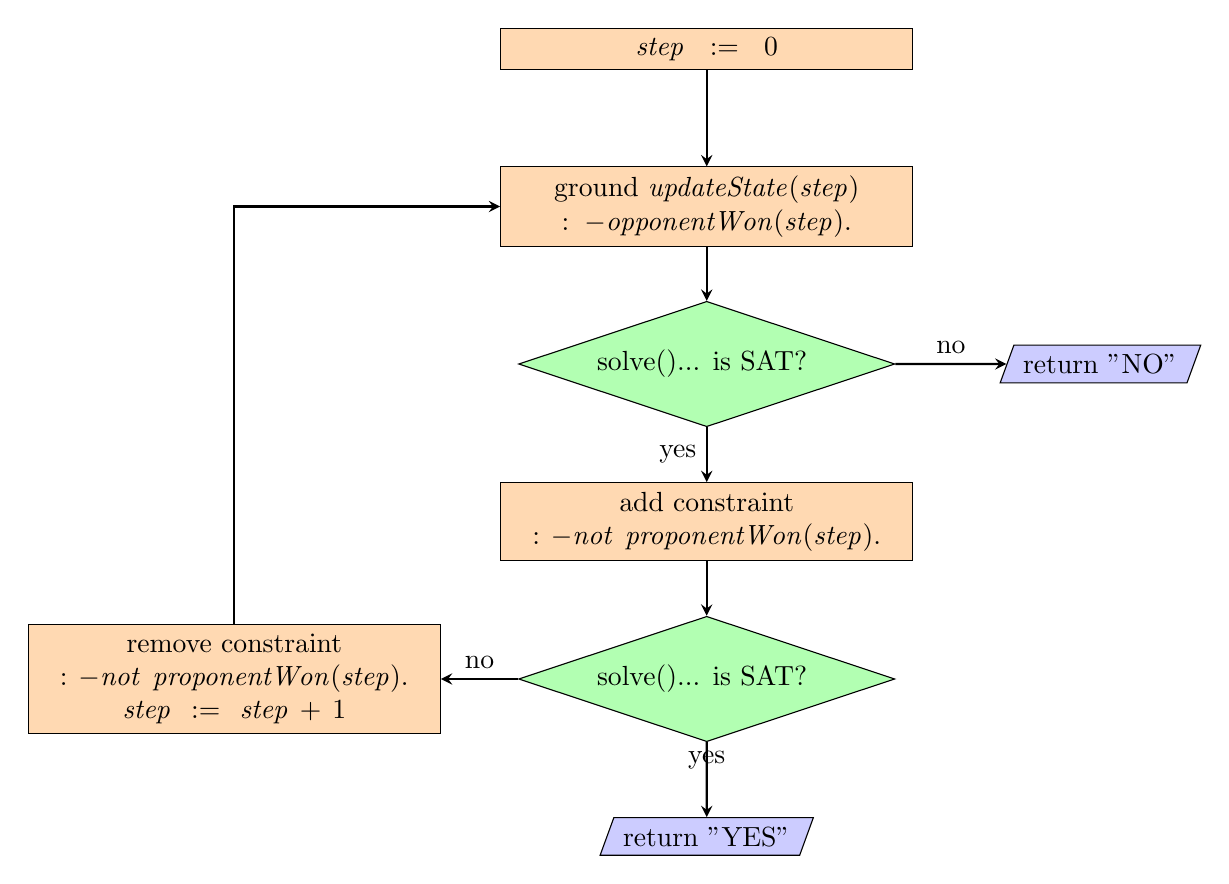
\begin{tikzpicture}[node distance=2cm,
        % styles
        startstop/.style = {
                rectangle, rounded corners,
                %minimum width=3cm, minimum height=1cm,
                text centered, draw=black, fill=red!30
            }, %
        io/.style = {
                trapezium, trapezium left angle=70, trapezium right angle=110,
                %minimum width=3cm, minimum height=1cm, 
                text centered, draw=black, fill=blue!20
            },
        decision/.style = {
                diamond, aspect=3,
                %minimum width=3cm, minimum height=1cm, 
                text centered, draw=black, fill=green!30
            },
        process/.style = {
                rectangle, text width=5cm,
                % minimum width=3cm, 
                %minimum height=1cm, 
                text centered, draw=black, fill=orange!30
            },
        arrow/.style ={
                thick,->,>=stealth
            }]

    %\node (start) [startstop] {Start};
    %\node (input) [io, below of=start] {input};
    \node (init) [process] { $\mathit{step}:=0$ };
    \node (update_state) [process, below of=init] { ground $\mathit{updateState(step)}$\\$:- \mathit{opponentWon(step)}.$ };
    \node (solve_1) [decision, draw, align=left, below of=update_state] { solve()... is SAT? };
    \node (game_over) [io, right of=solve_1, xshift=3cm] { return "NO" };
    \node (game_on) [process, below of=solve_1] { add constraint $:-\mathit{not}\;\mathit{proponentWon(step).}$ } ;
    \node (solve_2) [decision, draw, align=left, below of=game_on] { solve()... is SAT? };
    \node (prop_won) [io, below of=solve_2] { return "YES" };
    \node (game_on_2) [process, left of=solve_2, xshift=-4cm] { remove constraint $:-\mathit{not}\;\mathit{proponentWon(step).}$\\$\mathit{step} := \mathit{step} + 1$ } ;


    % % arrows
    \draw [arrow] (init) -- (update_state);
    \draw [arrow] (update_state) -- (solve_1);
    \draw [arrow] (solve_1) -- node[anchor=east] {yes} (game_on);
    \draw [arrow] (solve_1) -- node[anchor=south] {no} (game_over);
    \draw [arrow] (game_on) -- (solve_2);
    \draw [arrow] (solve_2) -- node[anchor=south] {no} (game_on_2);
    \draw [arrow] (solve_2) -- node[anchor=south] {yes} (prop_won);
    % \draw [arrow] (game_on_2.west) -- (update_state.west);
    \draw [arrow] (game_on_2) |- (update_state);

    % |- ($(A-2.south east)!0.5!(A-3.north east)$)
        %   -| ([xshift=7mm] A-3.north);

    % \draw [arrow] (input) -- (problem_supported);
    % \draw [arrow] (problem_supported) -- node[anchor=south] {no} (mu_toksia_task);
    % \draw [arrow] (problem_supported) -- node[anchor=east] {yes} (htd);
    % \draw [arrow] (htd) -- (tw_small);
    % \draw [arrow] (tw_small) -- node[anchor=south] {no} (mu_toksia_enum);
    % \draw [arrow] (mu_toksia_enum) -- (count_mu_toksia_enum);
    % \draw [arrow] (tw_small) -- node[anchor=east] {yes} (run_dpdb);
    % \draw [arrow] (run_dpdb) -- (output);
    % \draw [arrow] (count_mu_toksia_enum) |- (output);
    % \draw [arrow] (mu_toksia_task) |- (output);
    %\draw [arrow] (output) -- (stop);
\end{tikzpicture}
\end{document}